% Energy and Buildings (Elsevier) version.
% Build: latexmk -pdf main-enb.tex   (or: make enb)
% The text lives in sections/ and is shared with main-jbps.tex, so the paper
% can be moved to the Journal of Building Performance Simulation by building
% that file instead. Only the front matter and the reference style differ.
% Layout: review preprint (12 pt, wide margins) by default.
% main-enb-11pt.tex sets a tighter journal-like layout for page counts.
\providecommand{\enblayout}{preprint,12pt}
\expandafter\documentclass\expandafter[\enblayout,a4paper]{elsarticle}

% Shared preamble for both journal versions. Keep journal-specific settings
% in main-enb.tex / main-jbps.tex.
\usepackage[T1]{fontenc}
\usepackage[utf8]{inputenc}
\usepackage{lmodern}
\usepackage[british]{babel}
\usepackage{amsmath,amssymb}
\usepackage{graphicx}
\usepackage{booktabs}
\usepackage{tabularx}
\usepackage{array}
\usepackage{longtable}
\usepackage{siunitx}
\usepackage{textcomp}
\usepackage{newunicodechar}
\newunicodechar{°}{\textdegree}
\newunicodechar{²}{\textsuperscript{2}}
\newunicodechar{●}{\ensuremath{\bullet}}
\newunicodechar{−}{\ensuremath{-}}
\newunicodechar{±}{\ensuremath{\pm}}
\newunicodechar{·}{\ensuremath{\cdot}}
\newunicodechar{×}{\ensuremath{\times}}
\newunicodechar{≈}{\ensuremath{\approx}}
\usepackage{xcolor}
\usepackage{caption}
\usepackage[hidelinks]{hyperref}
\usepackage{xurl}

\sisetup{detect-all}
\setlength{\emergencystretch}{3em}
\renewcommand{\arraystretch}{1.15}
\newcolumntype{L}[1]{>{\raggedright\arraybackslash}p{#1}}
\newcolumntype{Y}{>{\raggedright\arraybackslash}X}

% Figures: drop updated files into figures/ with the same names.
% \includegraphics picks .pdf first, then .png.
\graphicspath{{figures/}}
\DeclareGraphicsExtensions{.pdf,.png,.jpg}

% Shows a framed placeholder when a figure file is not there yet,
% so the paper always compiles.
\newcommand{\paperfigure}[2][width=\linewidth]{%
  \IfFileExists{figures/#2.pdf}{\includegraphics[#1]{#2}}{%
  \IfFileExists{figures/#2.png}{\includegraphics[#1]{#2}}{%
  \fbox{\parbox[c][5cm][c]{0.9\linewidth}{\centering Figure file \texttt{figures/#2} not yet added}}}}}

\newcommand{\papertitle}{How much does filling gaps in weather data change building energy results? A hide-and-refill test}
\newcommand{\correspondingemail}{sanjay.somanath@chalmers.se}

\newcommand{\graphicalabstractslot}{%
  \IfFileExists{figures/graphical_abstract.pdf}{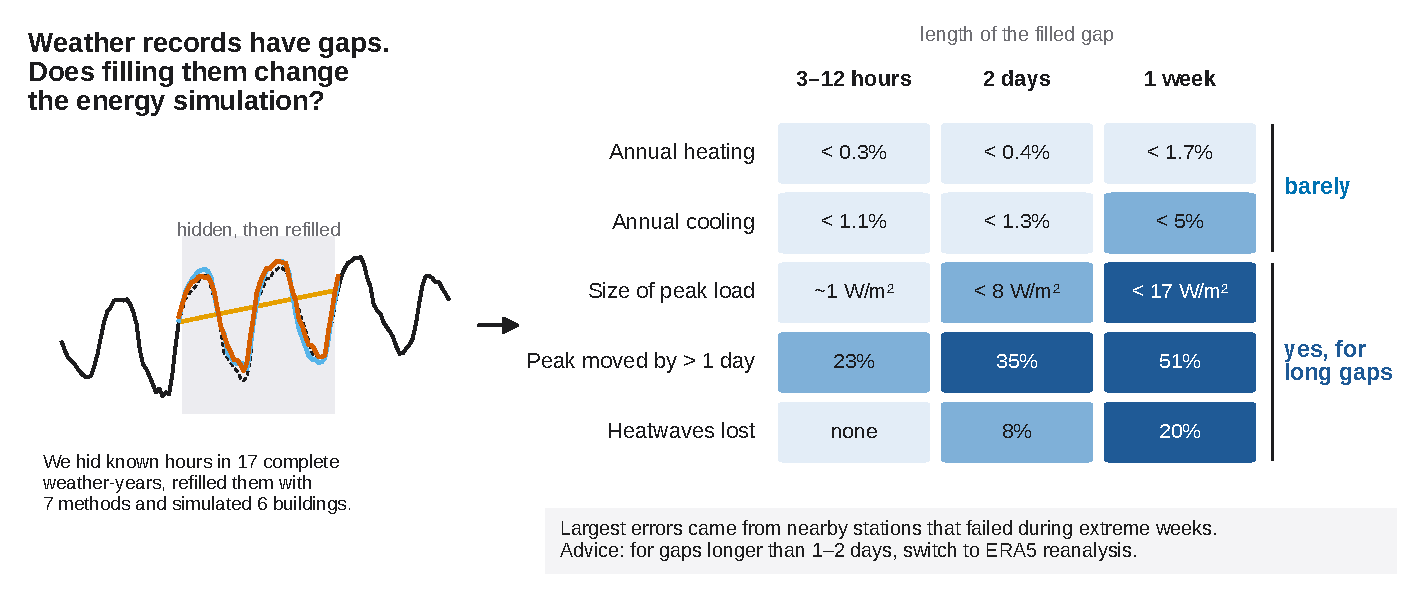
\includegraphics[width=\linewidth]{graphical_abstract}}{%
  \IfFileExists{figures/graphical_abstract.png}{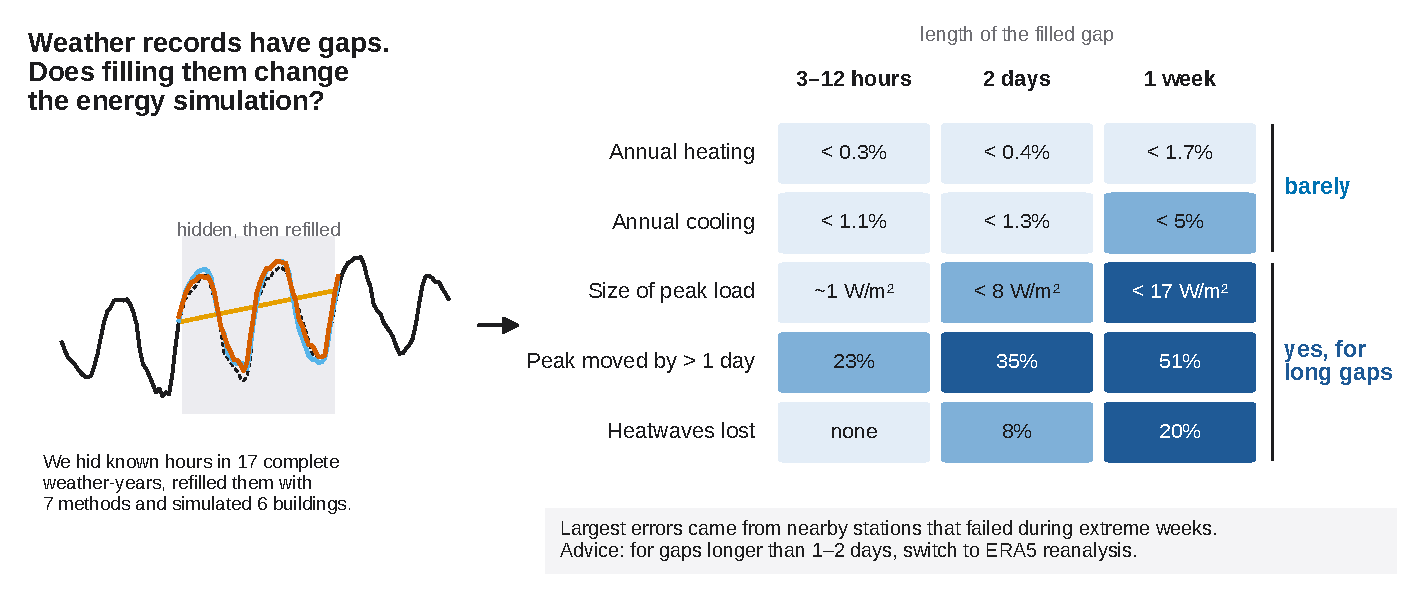
\includegraphics[width=\linewidth]{graphical_abstract}}{%
  \fbox{\parbox[c][6cm][c]{0.9\linewidth}{\centering Graphical abstract: add \texttt{figures/graphical\_abstract.pdf}\\(Elsevier: 1328 $\times$ 531 px or larger, readable at 5 $\times$ 13 cm)}}}}}


% Energy and Buildings uses numbered references in square brackets.
% For author-year citations instead, use: \biboptions{authoryear}
% together with \bibliographystyle{elsarticle-harv} below.
\biboptions{numbers,sort&compress}

\journal{Energy and Buildings}

\begin{document}

\begin{frontmatter}

\title{\papertitle}

\author[cth]{Sanjay Somanath\corref{cor1}}
\ead{\correspondingemail}
\author[cth]{Alexander Hollberg}
\cortext[cor1]{Corresponding author.}
\affiliation[cth]{organization={Department of Architecture and Civil Engineering, Chalmers University of Technology},
            city={Gothenburg},
            country={Sweden}}

\begin{abstract}
Weather files for a particular past year are built from station records, which almost always have gaps. Filling methods are usually judged against the weather, not by their effect on simulations. We hid known hours in 17 complete Swedish weather-years and refilled them with seven methods, from linear interpolation to a nearby station and the ERA5 reanalysis, including a stepwise method with and without a switch to ERA5 for long gaps. Gaps of 3 hours to one week fell at random or during heatwaves and cold spells, and six typical buildings were simulated. The results show that gap filling barely changes annual heating: with four 12-hour gaps a year, every method stayed within 0.3\% in 95\% of cases, and the extra heating followed the building's heat-loss coefficient times the temperature error summed over the gap. Peaks are more fragile. A filled extreme is usually milder than the real one, and the year's peak often has a near-equal day, so when a week-long gap hid the heating peak, the filled peak moved by over a day in half the cases. Which weather was hidden mattered more than the method; methods differed mainly in worst cases. These came from nearby stations that matched well in ordinary weather but not during a week-long extreme; switching to ERA5 after one or two days (three hours for solar radiation) avoided them. The tested gaps cover 99\% of the gaps in usable Swedish files. Filled hours should be reported, and peaks given with an uncertainty band.

\end{abstract}

% Graphical abstract and highlights are separate uploads at Elsevier and are not
% printed in the article, so the journal-look builds leave them out.
\providecommand{\showprelims}{1}
\if1\showprelims
\begin{graphicalabstract}
\graphicalabstractslot
\end{graphicalabstract}

\begin{highlights}
\item Judge a gap fill by its bias over the gap, not by its hourly error
\item Hiding and refilling known hours isolates the effect of gap filling on energy results
\item Gaps up to 12~h change annual heating by under 0.3\% in 95\% of cases
\item Half of peaks hidden by a week-long gap move by over a day, often to a near-equal day
\item In 2 of 510 week-long fills, a well-matched nearby station failed in an extreme

\end{highlights}
\fi

\begin{keyword}
weather data \sep gap filling \sep actual meteorological year \sep ERA5 \sep building energy simulation \sep peak load

\end{keyword}

\end{frontmatter}

\section{Introduction}\label{sec:1}

To check a building model against the energy bills of a particular year, a modeller needs that year's weather, hour by hour. Such actual meteorological years (AMYs) are used to compare models with measured energy use \citep{ashrae2014,steenenglund2020}, to study real heatwaves, and as the starting point for future weather files \citep{rodrigues2023}. The choice of weather file matters: another weather source can change annual energy use by about 7\% and monthly loads by about 40\% \citep{bhandari2012}, and differences between years affect peak demand more than annual energy \citep{hong2013}.

AMYs are made from weather-station records, and these records are rarely complete. In our survey of hourly Swedish station records, nearly half of all station-years, and a third of those complete enough to use, have at least one gap longer than two days. Every AMY therefore needs its gaps filled, whether by interpolation, by copying from nearby stations, by using a global weather model, or by statistical methods \citep{wilcox2008,korner2018,smith2021}.

Gap-filling methods are usually judged by how closely they match the missing weather \citep{korner2018,nrel2021,ieapvps2023,jacobs2024}, and studies of weather files compare whole files, not the filled hours within one. A modeller therefore has no evidence on whether a filled gap changes annual heating, moves a peak load, or removes the heatwave the year was chosen for. The choice of source is also open. A nearby station records the same weather systems, but local effects such as a sea breeze or cold air collecting in low ground can set it apart \citep{miller2003,daly2010}; a global weather model such as ERA5 is always available but smooths the hottest and coldest hours \citep{lopes2024}. Which weakness matters more for simulation results, and for how long a local source can be trusted, is not known.

This paper measures how filling gaps in weather data changes building simulation results. We ask two questions:

\begin{enumerate}
\item
  How do the length, type (general weather or solar) and timing of a gap affect annual heating and cooling, peak loads, the timing of peaks, and heatwaves?
\item
  Which filling sources work best, and up to what gap length?
\end{enumerate}

We test gaps of 3 hours to one week, which cover 99\% of the gaps and about two thirds of the missing hours in Swedish records complete enough to make an AMY. We carry the hide-and-refill test, common in studies of gap filling, through to building simulation results: we measure how the length, type and position of a gap, and the filling method, change these results in 17 Swedish weather-years and six typical buildings, and we compare the methods by their worst case as well as their typical error. A heatwave year shifted to a future climate serves as a stress test.

\section{Background}\label{sec:2}

Hourly station records lose data for many reasons, from a failed sensor to a station being moved, and how a gap is filled depends mostly on its length. Four kinds of method are in common use (Table~\ref{tab:1}): simple methods work well for short gaps, while long gaps need another source of data.

\begin{table*}[tbp]
\centering
\small
\caption{Common kinds of gap-filling method.}
\label{tab:1}
\begin{tabular}{@{}L{\dimexpr0.232\linewidth-2\tabcolsep}L{\dimexpr0.116\linewidth-2\tabcolsep}L{\dimexpr0.174\linewidth-2\tabcolsep}L{\dimexpr0.159\linewidth-2\tabcolsep}L{\dimexpr0.319\linewidth-2\tabcolsep}@{}}
\toprule
Kind of method & Typical use & Strength & Weakness & Examples \\
\midrule
Filling over time & Gaps of a few hours & Simple; uses only the station's own record & Smooths out peaks; fails after about a day & Linear interpolation and curve fitting; TMY3 filling of 6--47 hour gaps \citep{wilcox2008}; solar interpolation \citep{nrel2021} \\
Copying from a nearby station & Hours to weeks & Uses real measurements of the same weather & Needs a similar station close by; local differences & Nearby-station correction \citep{henn2013,eguiaoller2017} \\
Global weather models and satellites & Any length, even a whole missing variable & Always available and physically consistent & Averages over a large area; misses local extremes & ERA5 \citep{hersbach2020}; satellite solar data \citep{babar2019} \\
Statistical and machine-learning methods & Hours to weeks & Learns links between variables and stations & Needs training data; hard to check & Gradient boosting \citep{korner2018}; neural networks \citep{meshkinkiya2020,xie2021} \\
\bottomrule
\end{tabular}
\end{table*}

\subsection{Filling methods and tools}\label{sec:2.1}

Linear interpolation is the usual choice for short gaps. The US TMY3 files fill gaps of 6 to 47 hours with curves \citep{wilcox2008}, and for measured solar radiation linear interpolation was the best of eight methods \citep{nrel2021}. Methods based on typical daily patterns stretch this to a day or two. The diyepw tool, which makes EnergyPlus AMY files from US station data \citep{smith2021}, interpolates gaps of up to 6 hours, fills gaps of up to 48 hours with the average of the same hour over the four weeks around the gap, and rejects longer ones \citep{diyepw2023}. For hourly air temperature, the best method depends on the gap length and on how many nearby stations there are \citep{henn2013,hu2014}.

Copying from a nearby station keeps real weather events, but a station that differs in height, exposure or distance from the sea can be biased unless the match is checked. \citet{eguiaoller2017} estimated a full year of weather at each of 18 stations from the stations around it and simulated a dwelling with each: universal kriging gave errors of about 10\% in annual heating and 7\% in the heating peak, against 27.5\% and 17\% for the nearest station. Kriging with a height term cut the hourly temperature error by about a third against the nearest station \citep{rosillon2024}, and a nearby station beat ERA5-Land only where the two were well correlated \citep{sirpapoma2025}.

\subsection{Global weather models and learned methods}\label{sec:2.2}

ERA5 is a global weather model with hourly values on a grid of about 31~km, from 1940 onwards \citep{hersbach2020,soci2024}. It has no gaps, but each value is an average over a large area. Its daily temperature range is too small \citep{lopes2024}, and its solar radiation is too high under cloud and slightly too low under clear skies, worse on coasts and in mountains \citep{urraca2018}, although hourly errors largely cancel over a month \citep{babar2019}. In built-up areas of the UK the related ERA5-Land misses many of the hottest hours, yet remains a reliable stand-in for building simulation \citep{yu2026}. Comparisons of filling methods agree that linear interpolation is best for short gaps and a model or satellite source for longer ones, for solar radiation \citep{ieapvps2023} and for air temperature, where ERA5 corrected to the station did best beyond about five hours \citep{jacobs2024}. A US database of hourly weather for energy modelling likewise moves from a nearby station to the MERRA-2 reanalysis as gaps grow \citep{wang2024}, and \citet{lundstrom2012} combined measured weather with modelled solar radiation to make AMY files for northern Europe.

Learned methods can be more accurate. Gradient boosting filled hourly gaps in temperature, wind and humidity at German stations with median errors of about 0.7~°C, 0.8~m/s and 4\% relative humidity, better than neural networks or linear regression \citep{korner2018}. Neural networks trained on nearby stations filled temperature and humidity well for building simulation in Milan \citep{meshkinkiya2020}, and a deep-learning method filled gaps of 30 and 60 days in half-hourly temperature records with errors that did not grow with gap length \citep{xie2021}. None of these studies, and none of the tools above, reports how its gap filling changes simulated energy use, peaks or their timing.

\subsection{Why simple methods, with their error measured}\label{sec:2.3}

Extremes at a station are often set by local processes such as a sea breeze or cold air collecting in low ground \citep{miller2003,daly2010}. A few stations tens of kilometres apart and a global model on a 31~km grid do not capture these, so more complex methods have little extra information at the hours that matter most. Any method that gives one best estimate, including regression and machine learning trained on the average error, makes extremes too mild \citep{begueria2019}, and a single filled value hides its uncertainty \citep{little2019}. We therefore test simple methods that need no training and can be used anywhere, and measure the error they leave in simulation results.

\subsection{How the weather file affects simulation results}\label{sec:2.4}

The choice of weather file is known to change annual energy use by several per cent and peak loads by much more. These known differences give a scale for judging whether the errors from gap filling matter (Table~\ref{tab:2}).

\begin{table*}[tbp]
\centering
\small
\caption{How the choice of weather file changed simulation results in earlier studies.}
\label{tab:2}
\begin{tabular}{@{}L{\dimexpr0.219\linewidth-2\tabcolsep}L{\dimexpr0.324\linewidth-2\tabcolsep}L{\dimexpr0.172\linewidth-2\tabcolsep}L{\dimexpr0.284\linewidth-2\tabcolsep}@{}}
\toprule
Study & What was compared & Effect on annual energy & Effect on peaks or shorter periods \\
\midrule
\citet{hong2013} & 30 actual years against a typical year, 17 US climate zones, 3,162 simulations & The typical year can be well above or below the 30-year average & Year-to-year weather affects peak demand more than energy use \\
\citet{bhandari2012} & Commercial weather sources against a local station & About ±7\% & Monthly loads about ±40\% \\
\citet{daneshfar2023} (preprint) & Older and newer typical years against actual 2006--2015 weather & −4.2\% to +53.3\% & Peak load up to −49.4\% (older typical year) and −31.5\% (newer) \\
\bottomrule
\end{tabular}
\end{table*}

Typical years, such as TMY, TRY and IWEC files, represent long-term average weather and leave out extremes \citep{wilcox2008,herrera2017}. Actual years are needed to compare models with measured energy use \citep{steenenglund2020}, to study a specific heatwave and to look at differences between years. Weather matters more in colder climates \citep{hong2013}, and peak loads and short periods vary far more than annual energy: a typical year was a poor basis for peak loads \citep{daneshfar2023}, and monthly loads varied about six times as much as annual loads \citep{bhandari2012}. An error in a few filled hours may likewise vanish in an annual total yet dominate a peak.

Extreme years are used to study overheating and cooling peaks. \citet{nik2016} made one typical and two extreme years for housing in Stockholm, \citet{porritt2012} used the 2003 heatwave to rank ways of reducing overheating in UK dwellings, UK design summer years are chosen by how severe their warm spells are \citep{eames2016}, and \citet{machard2020} built future heatwave files, noting that monthly morphing smooths out daily extremes. In such a year, a filled gap over the few hottest hours can remove the heatwave the year was chosen for.

\subsection{The research gap}\label{sec:2.5}

We searched Scopus and Web of Science in November 2026 and kept 82 papers (\ref{app:B}): 27 build or fill weather files, 36 compare filling methods against measured weather, and 19 measure how differences between weather files change simulated loads.

Earlier work compares whole weather files, or judges filling methods against the weather, but rarely follows the filled hours into a simulation. Uncertainty analysis is well established in building simulation, for inputs such as material properties, design choices, operation and weather \citep{hopfe2011,tian2013,wang2012}, yet filled weather hours are not treated as an uncertain input, although uncertainty and extreme events are named among the new challenges for weather files \citep{herrera2017}. Gap-filling studies judge methods against the weather only, including the two that fill temperature gaps from ERA5 corrected to the station \citep{lompar2019,jacobs2024}. The few that link filling to simulated energy use each cover one kind of filling (Table~\ref{tab:3}): two interpolate three-hourly records to hourly ones and look at ventilation or air-conditioning energy \citep{anjomshoaa2019,liu2022}, one estimates whole records from surrounding stations and reports the heating peak of one dwelling \citep{eguiaoller2017}, and one fills measured indoor temperatures, not weather \citep{titikpina2015}. None hides real gaps of several lengths in actual-year data, refills them with several methods, including nearby stations and a global weather model, and measures the change in annual demand, peak size and peak timing across buildings and climates. This paper carries the established hide-and-refill test through to these results, with the differences between whole files in Table~\ref{tab:2} as a scale.

\begin{table*}[tbp]
\centering
\footnotesize
\caption{The closest earlier studies and this one.}
\label{tab:3}
\begin{tabular}{@{}L{\dimexpr0.148\linewidth-2\tabcolsep}L{\dimexpr0.344\linewidth-2\tabcolsep}L{\dimexpr0.247\linewidth-2\tabcolsep}L{\dimexpr0.261\linewidth-2\tabcolsep}@{}}
\toprule
Study & What was filled & Filling methods compared & Building results measured \\
\midrule
\citet{titikpina2015} & Gaps of 10 to 424 hours in measured indoor temperatures of four offices in one monitored building & One random-sampling method that keeps each gap's daily pattern; no comparison & Simulated heating energy of the monitored zone (TRNSYS), over 4,000 runs \\
\citet{eguiaoller2017} & A full year of hourly weather (six variables) at each of 18 stations in north-west Spain, estimated from the stations around it & Five: nearest station, three kinds of kriging and thin-plate splines & Simulated heating demand and heating peak of one dwelling at each site (TRNSYS) \\
\citet{anjomshoaa2019} & Three-hourly records turned into hourly ones, for heating and cooling seasons separately (Kerman, Iran) & Linear interpolation and cubic spline, each with two humidity variables & Calculated heating and cooling energy for fresh air in a ventilation unit \\
\citet{liu2022} & Hourly temperature, humidity and wind from three-hourly values, in the hottest and coldest weeks (three Chinese coastal cities) & Five interpolation methods & Simulated air-conditioning energy (EnergyPlus) of weather with added errors sized to match the interpolation errors \\
\citet{jacobs2024} & Gaps of 1 hour to 2 weeks in urban and rural air temperature records (Turku, Finland) & Five: linear interpolation, ERA5, and three ways of correcting ERA5 to the station & None; judged against the weather and the urban heat island \\
\citet{wang2024}, CHUWD-H & Gaps in hourly records at 550 US stations, 1998--2020 & A multi-step order using a nearby station and reanalysis, against three simpler methods & None; judged against the weather \\
This study & Hidden gaps of 3 hours to one week in 17 Swedish actual years, general weather and solar radiation separately & Eight methods, including a checked nearby station, ERA5 and a stepwise method & Annual heating and cooling, peak size and timing, and heatwaves kept, for six buildings \\
\bottomrule
\end{tabular}
\end{table*}

\section{Weather data and gaps in Swedish records}\label{sec:3}

SMHI publishes hourly observations from 158 stations that record all five weather variables a weather file needs, but the records have gaps: hours, days and sometimes more than a month are missing (Section~\ref{sec:3.3}). We built the weather files with smhi2epw, our open-source tool that makes actual-year EnergyPlus weather files (EPW) for any place in Sweden from 1999 (see Data and code availability); how it downloads ERA5 and checks each finished file is described in \ref{app:A}.

\subsection{Data sources and solar radiation}\label{sec:3.1}

Five weather variables are required: air temperature, relative humidity, wind speed, wind direction and air pressure. They come from hourly observations at SMHI weather stations \citep{smhi2026a}. Solar radiation comes from STRÅNG, SMHI's model of solar radiation over Sweden \citep{landelius2001}. Where a station that measures solar radiation lies within 50~km, its measurements are used to correct the model. ERA5 values for the same year are taken at the main station, with a correction for height; the nearest ERA5 grid point lies 3.5--17~km from the station.

\subsection{The stepwise filling order}\label{sec:3.2}

Missing weather values are filled in a fixed order of steps, which we call the stepwise method. Each step fills only what the step before could not, and measured values are never changed. The order has one open choice for each type of gap: the gap length beyond which it skips the local steps and goes straight to ERA5. We test several lengths (Section~\ref{sec:4.4}) and report which works best as a result (Section~\ref{sec:5.6}).

\begin{enumerate}
\item
  \textbf{Measured values} from the main station.
\item
  Linear interpolation for gaps of up to three hours. Where a gap has a measured value on one side only, that value is held flat. Wind direction is filled by its compass components so that it does not swing the wrong way round.
\item
  Checked nearby stations within 75~km, at most three, nearest first, for gaps up to the switch-over length. For each gap and variable, the nearby station is compared with the main station over the 30 days either side of the gap and tested on 3 left-out days; a fixed correction is kept only if it cuts the error by at least 10\%. A station is rejected if its typical error on the left-out days is more than 3~°C, 15\% relative humidity, 3~m/s, 45° or 5~hPa. These loose limits remove only clearly unsuitable stations; those that passed usually matched much better, with a typical temperature error of 1.0~°C (90\% below 2.1~°C). \ref{app:C} tests stricter temperature limits.
\item
  \textbf{Typical daily patterns} for gaps of up to 48 hours. The pattern is taken from the nearest complete days within a week on each side and adjusted to meet the measured values at both ends of the gap. This step is our own; it is similar in aim to the four-week average used by diyepw (Section~\ref{sec:2.1}).
\item
  ERA5 for the same year and place, for anything still missing and for every gap longer than the switch-over length (Figure~\ref{fig:1}).
\end{enumerate}

Solar radiation is filled without nearby stations: first measured radiation, then STRÅNG, then linear interpolation for short gaps, then ERA5. The length of a solar gap is measured before night hours are set to zero, so that night does not split a long gap into short daytime pieces. For general weather we test switching to ERA5 after one day, after two days, or never; with test gaps of 3, 12, 48 and 168 hours, a one-day switch acts on the same gaps as a 12-hour one. For solar gaps we test switching after 3, 12 or 48 hours. The order with no switch is called the stepwise method with no switch.

\begin{figure*}[tbp]
\centering
\paperfigure{fig01}
\caption{The stepwise method fills short gaps from measurements and switches to ERA5 once a gap is longer than two days (general weather) or three hours (solar radiation). Each bar shows the gap lengths a source may fill; the gap-length axis is logarithmic. Sources are tried from the top, and an hour one source cannot fill falls to the next. The light bar is ERA5 filling any hour still empty. The grey dashed bars are used only without the switch (stepwise, no switch). Switching at one day for general weather and at 12 and 48 hours for solar radiation was also tested (Section~\ref{sec:5.6}).}
\label{fig:1}
\end{figure*}

\subsection{Gaps in Swedish station records}\label{sec:3.3}

Most real gaps are short, but most missing hours sit in a few very long gaps, mostly in records that are hardly usable (Figure~\ref{fig:2}). Of the 3,545 station-years from the 158 SMHI stations that report all five required variables in 1999--2025, 2,550 from 122 stations report every hour; the rest report every three hours, hold very little data or lack a variable.

Half of all missing hours sit in 7\% of the station-years. In 224 station-years (39 stations, 1999--2012), relative humidity is more than 95\% missing while the other variables are mostly present; these hold 42\% of all missing hours. A station's first or last year, often only partly covered, holds another 20\% (212 part-years). No station-year is missing for the whole year in every variable.

\begin{figure*}[tbp]
\centering
\paperfigure{fig02}
\caption{Most gaps are short, but most missing hours sit in long gaps, and many of these lie in records that are hardly usable. Each bar splits all gaps, or all missing hours, by gap length, in hourly SMHI station records for 1999--2025 (2,550 station-years from 122 stations). A gap is a run of missing hours in one variable. Usable files are station-years with at most 10\% of values missing (2,213 station-years). The number on the right is the share made up of gaps up to one week, the lengths tested in this study.}
\label{fig:2}
\end{figure*}

In the files a modeller would actually use, the picture is very different. In the 2,213 usable station-years (87\%, from 115 stations), gaps of up to a week hold 63\% of missing hours, and 90\% lie in gaps shorter than about 40 days. A third of these files have a gap longer than two days, and 15\% one longer than a week, mostly in wind or humidity: only 5\% have a temperature gap longer than two days. Over half (1,378, or 54\%) have at most 1\% missing and no gap over 48 hours. Gaps in a single variable make up 10\% of gaps and 6\% of missing hours, and winter has the most missing hours (1.91 million, against 0.7--1.1 million in each other season).

Gaps of up to a week, the lengths tested here, therefore cover 99\% of the gaps and about two thirds of the missing hours in usable files. Most of the remaining missing hours sit in records with too little measured weather to make an AMY at all: a station that started in November gives mostly a model year, better replaced by a reanalysis or typical year than filled. A year that lacks only humidity is different. With temperature, wind, pressure and sun measured, it is close to complete for heating and cooling, which depend on humidity only through sky radiation (Section~\ref{sec:4.3}), and its humidity can be filled from ERA5, with care where humidity itself matters, such as latent loads, moisture or comfort.

\section{Experiment design}\label{sec:4}

We take complete weather years, remove some known observations, fill them back in with each method, and simulate the same buildings with the complete and the filled weather. The buildings, the hours outside the gap and the simulation software are identical in each pair, so any difference in the results is caused by the gap and how it was filled (Figure~\ref{fig:3}).

\begin{figure*}[tbp]
\centering
\paperfigure{fig03}
\caption{Every filling method fills the same hidden hours in the same reference years, so each test file differs from its reference only in the filled gaps. The methods are described in Section~\ref{sec:4.4}.}
\label{fig:3}
\end{figure*}

\subsection{Reference weather}\label{sec:4.1}

We used six regions, from south to north (Malmö, Gothenburg, Stockholm, Östersund, Luleå and Kiruna), and three contrasting years: 2018 (hot, sunny and dry; \citealp{smhi2018}), 2021 (close to the 1991--2020 average) and 2023 (wet in the south, with a cold December). Seventeen of the 18 region-years had a suitable station (Figure~\ref{fig:4}). Kiruna 2018 had no station within 100~km that was complete enough. A reference year could have at most 1\% missing values and no gap longer than 48 hours. Its few small gaps were filled once and then kept the same in every case. Only real, quality-checked measurements were removed and scored.

\begin{figure*}[tbp]
\centering
\paperfigure{fig04}
\caption{The six study regions and the stations behind each reference year. Lines join each main station to its nearby station and its solar station. In (g) the years label the lines, because the main station changes from year to year. Kiruna 2018 had no station that met the data requirements.}
\label{fig:4}
\end{figure*}

\subsection{Buildings}\label{sec:4.2}

We used six typical Swedish buildings from the epsm\_data catalogue (version 0.7.0; Table~\ref{tab:4}), which, like the TABULA typologies \citep{loga2016} and the Swedish ECCABS model \citep{mata2013}, describes buildings by type and construction period. Walls, roofs and floors are layered from real materials in Boverket's database, and each building has window areas by direction, air leakage, ventilation typical of its period and standard Swedish patterns of use \citep{sveby2012}, all in its unrenovated state.

\begin{table*}[tbp]
\centering
\small
\caption{The six buildings, from the epsm\_data catalogue.}
\label{tab:4}
\begin{tabular}{@{}L{\dimexpr0.299\linewidth-2\tabcolsep}L{\dimexpr0.214\linewidth-2\tabcolsep}L{\dimexpr0.316\linewidth-2\tabcolsep}L{\dimexpr0.171\linewidth-2\tabcolsep}@{}}
\toprule
Building (catalogue name) & Built & Walls, windows and ventilation & U-values (W/m²K) \\
\midrule
Single-family house (sf\_se02) & 1961--75 & Timber frame; natural ventilation & Wall 0.31, window 2.30 \\
Single-family house (sf\_se06) & 2006--21 & Timber frame; balanced ventilation with heat recovery (75\%) & Wall 0.20, window 1.30 \\
Apartment block (mf\_se02) & 1961--75 (Million Programme) & Brick and timber; exhaust ventilation & Wall 0.42, window 2.22 \\
Apartment block (mf\_se06) & 2006--21 & Concrete with 220~mm insulation; heat recovery (75\%) & Wall 0.16, window 1.50 \\
Office (office\_se06) & 2006--21 & Concrete; heat recovery; window area raised from 30\% to 60\% of the wall to represent a highly glazed office & Wall 0.18, window 1.30 \\
School (school\_se03) & 1976--85 & Timber frame; supply and exhaust ventilation & Wall 0.34, window 2.25 \\
\bottomrule
\end{tabular}
\end{table*}

Heating and cooling are modelled as ideal systems with unlimited capacity and no humidity control. Results are the heat that must be added or removed to keep the set temperatures, including the heating or cooling of ventilation air. The ground floor sits on a fixed 18~°C boundary in every case. This changes absolute demand. It cancels out of the differences in kWh/m² between pairs, but it does affect percentage errors, because it changes the share of demand that depends on the weather.

\subsection{Test gaps}\label{sec:4.3}

We created two types of gap: \textbf{general weather gaps}, where all five required variables are removed at once, and \textbf{solar gaps}, where solar radiation is removed. Each type was tested with gaps of 3, 12, 48 and 168 hours (one week), placed in two ways:

\begin{itemize}
\item
  \textbf{Random seasonal gaps.} Three random draws each place one gap in winter, spring, summer and autumn, so a file loses 12, 48, 192 or 672 hours in total.
\item
  \textbf{Extreme-event gaps.} One gap per file, centred on the hottest or coldest hour of the year, or on the hottest hour of a heatwave or coldest hour of a cold spell, where these exist. Where the hottest hour of a heatwave was also the hottest hour of the year, or the coldest hour of a cold spell the coldest of the year, the two layouts hide the same hours; such gaps are counted once (91 of 230 event gaps).
\end{itemize}

In a solar gap, the measured total radiation and STRÅNG's total, direct and diffuse radiation are all removed for the hidden hours. The true value for scoring is the measured total where a solar station lies within 50~km, otherwise STRÅNG's total; the direct and diffuse parts are always STRÅNG's, so they are modelled, not measured. Methods that work from the hours either side of the gap fill total radiation and then split it into direct and diffuse parts (Erbs--Driesse), while ERA5 provides all three parts from an independent model.

Figure~\ref{fig:5} shows both layouts. Gap positions were chosen from the weather alone, never from the simulation results. Each method filled the gaps without seeing the removed values, and everything outside the gaps was exactly the same as the reference.

We did not test gaps in relative humidity alone, although humidity has the most long gaps in Swedish records, many of them in nearly empty humidity records (Section~\ref{sec:3.3}). With ideal heating and cooling and no humidity control, humidity affects the heating and cooling we report only through the sky radiation that is calculated from the dew point. The error from a gap in all five variables is therefore expected to be larger than that from a humidity-only gap.

\begin{figure*}[tbp]
\centering
\paperfigure{fig05}
\caption{Gaps are placed once per season in three random draws, or once per file at a weather event. Gaps of 3 and 12 hours are drawn wider than to scale so they stay visible. General weather and solar gaps are hidden in separate files. Winter is December to February. Event hours (b) are the warmest and the coldest measured hour, the hottest hour of a heatwave and the coldest hour of a cold spell, where these occur.}
\label{fig:5}
\end{figure*}

\subsection{Methods compared}\label{sec:4.4}

The eight methods run from linear interpolation, which needs nothing but the hours either side of the gap, to ERA5 only, which ignores the station altogether; nearby stations, daily patterns and the stepwise order lie in between (Table~\ref{tab:5}).

\begin{table*}[tbp]
\centering
\small
\caption{The gap-filling methods compared. A dot shows that a method was tested on that type of gap: general weather (all five variables hidden together) or solar radiation.}
\label{tab:5}
\begin{tabular}{@{}L{\dimexpr0.234\linewidth-2\tabcolsep}C{\dimexpr0.108\linewidth-2\tabcolsep}C{\dimexpr0.139\linewidth-2\tabcolsep}L{\dimexpr0.518\linewidth-2\tabcolsep}@{}}
\toprule
Method & General weather & Solar radiation & What it does \\
\midrule
Stepwise & ● & ● & Linear interpolation up to 3 hours, then a checked nearby station and daily patterns, then ERA5. General weather gaps longer than two days and solar gaps longer than three hours go straight to ERA5. Solar gaps skip the nearby station \\
Stepwise, no switch & ● & ● & As the stepwise method, but the local steps are used for gaps of any length (daily patterns for solar gaps of up to 48 hours) \\
Stepwise, patterns first & ● & -- & As the stepwise method with no switch, but daily patterns before nearby stations \\
Interpolation then patterns & ● & ● & Linear interpolation up to 3 hours, then daily patterns up to 48 hours; longer gaps are not filled \\
Nearby station & ● & -- & A fixed nearby station for every hidden hour, after checking it against the main station \\
ERA5 only & ● & ● & ERA5 for every hidden hour \\
Four-week average & ● & ● & The rules of the diyepw tool: linear interpolation up to 6 hours; for 7--48 hours, the average of the same hour of day over the four weeks around the gap; longer gaps from ERA5 \\
Linear interpolation only & ● & ● & Interpolated between the values either side of the gap, however long \\
\bottomrule
\end{tabular}
\end{table*}

Table~\ref{tab:5} lists the eight methods, and Figure~\ref{fig:6} shows how each fills a gap. The nearby station and the stepwise method with patterns first apply only to general weather gaps, as solar radiation is never copied from nearby stations. The two stepwise orders with no switch use the same stations, data and checks, so comparing them shows the effect of the order alone. The four-week average follows diyepw version 1.3.1 (Section~\ref{sec:2.1}), except that it fills relative humidity rather than dew point, is also applied to solar radiation, and fills gaps longer than 48 hours from ERA5 instead of rejecting them. Each file holds one type and length of gap, so the results for each switch-over length are taken from the runs of the stepwise method with no switch and of ERA5 only; on one region-year, code with the switch gave identical files. Each switch-over length is judged by its worst case and its 95th-percentile regret, and checked on held-out years (Section~\ref{sec:5.6}). Unless stated otherwise, Section~\ref{sec:5} reports a two-day switch for general weather and a three-hour switch for solar gaps.

\begin{figure*}[tbp]
\centering
\paperfigure{fig06}
\caption{How each method filled one real 48-hour gap: Stockholm-Arlanda, 20--22 April 2023 (shaded), from the experiment. Black: measured values. Dashed: the hidden true values. Coloured: the filled values, in the colour each method has in every figure. Light grey in (d) and (e): that source outside the gap. (a) Linear interpolation. (b) Daily patterns. (c) The four-week average, the rule used by diyepw. (d) The nearby station, Stockholm-Bromma 30~km away, shifted by −0.9~°C after its check. (e) ERA5. (f) The stepwise method, which here used the nearby station because it passed its checks; Figure~\ref{fig:1} gives the full order. The number in each panel is the mean absolute error over the 48 hidden hours.}
\label{fig:6}
\end{figure*}

\subsection{Results compared}\label{sec:4.5}

For each building and gap we compare the filled case with its reference. Peak results are reported only where the reference annual peak fell inside the gap, because a peak outside the gap says nothing about the filling. A random gap rarely contains the peak (0--7\% of building results), so peak results come from the gaps centred on events. To see where in the year errors arise, we split each file's annual error between its four seasonal gaps, using the change in load during each gap and the week after it; these add up almost exactly to the annual error. We compare:

\begin{itemize}
\item
  Annual heating and cooling demand (kWh/m² and \%). Cooling percentages are only given where reference cooling is at least 1~kWh/m².
\item
  The size of the annual peak heating and cooling load (W/m²), where the peak fell inside the gap.
\item
  The timing of the peak: whether the peak hour stays the same, and if not, how far it moves.
\item
  The average hourly load error inside the gap and in the week after it, and over the whole year.
\item
  The weather error in the filled hours.
\item
  Heatwaves (at least three days in a row with a daily maximum of 25~°C or more) and cold spells (at least three days in a row with a daily minimum of −10~°C or lower): whether their dates, length and peak temperature are kept. SMHI uses the 25~°C limit but requires five days in a row \citep{smhi2026b}; we use three so that enough events occur, and also report the five-day definition. Fixed limits are rarely reached in some places, so we also use local definitions: a warm spell has a daily maximum above the 95th percentile of that place's summer maxima, and a relative cold spell a daily minimum below the 5th percentile of its winter minima, each for at least three days.
\end{itemize}

\subsection{Size of the experiment and checks}\label{sec:4.6}

The experiment is large enough to show worst cases as well as typical ones: 34,236 building results from 15,390 separate simulations, as identical weather files share one simulation.

The percentiles in Section~\ref{sec:5} describe the cases we tested. They are not confidence intervals, because the six buildings share each weather gap and so are not independent samples. Each 95th percentile for random seasonal gaps rests on 306 building results from 51 filled files. To show how much the results depend on the region-years chosen, we resampled the 17 region-years 1,000 times and report the 95\% range of the resampled 95th percentiles. For four week-long general weather gaps filled by the stepwise method, the heating error was 1.7\%, with a range of 0.8--2.4\%.

To see what makes one case worse than another (Section~\ref{sec:5.7}), we fitted a linear model to the logarithm of the size of each annual error, with gap length, placement, building, region-year and method as factors, plus three pairs of factors (gap length with method, gap length with placement, building with region-year); a factor's share is the drop in fit when it is left out. We repeated the fit with each hidden window (region-year and gap position) as a factor, and with the summed temperature error as a further term. To relate weather error to load error (Section~\ref{sec:5.8}), we fitted, for each building, a line through zero between the change in heating over each 48-hour or week-long gap and the following week and the temperature error summed over the gap in °C·days, separately for gaps starting in October to April and in May to September. We checked it against a fit with an intercept and against fits for each gap length, and compared each slope with the building's heat-loss coefficient. For peaks and cooling we used a simpler fit, with one point per filled file, against the average temperature and humidity errors over the gap, and for solar gaps the summed error in total radiation.

\subsection{Software, settings and computing}\label{sec:4.7}

The buildings are simulated in EnergyPlus \citep{crawley2001} through EPSM, our research group's open-source software for simulating building stocks \citep{sbchalmers2026}. Each building model is identical across all weather methods for a given region and year, and this is checked automatically. Table~\ref{tab:6} lists the software and settings.

\begin{table*}[tbp]
\centering
\small
\caption{Software, settings and computing.}
\label{tab:6}
\begin{tabular}{@{}L{\dimexpr0.347\linewidth-2\tabcolsep}L{\dimexpr0.653\linewidth-2\tabcolsep}@{}}
\toprule
Item & Setting \\
\midrule
Simulation engine & EnergyPlus 24.2.0 (ideal loads) \\
EPSM Core & 0.9.1; EPSM 0.5.1; epsm\_data 0.7.0 \\
smhi2epw & 1.3.0, pvlib 0.16.1 (SPA geometry, Erbs--Driesse); Python 3.12.3, NumPy 2.5.4, pandas 3.0.6 \\
Campaign code & epsm\_studies study scripts and exact commits, archived with the campaign outputs (see Data and code availability) \\
Run period & Full calendar year, hourly results, local standard time (UTC+1) with no summer time \\
HVAC & Ideal loads, unlimited capacity, no humidity control \\
Ground boundary & Ground floor held at a constant 18~°C \\
Outputs kept & Hourly heating and cooling loads, annual totals, peaks (with every hour that ties for the peak), and a record file and error log for each run \\
Weather cases & 904 gap layouts; 6,328 planned weather cases, of which 5,689 were run (387 needed a method that does not apply, such as a nearby station for a solar gap, and 252 had no nearby station that passed the checks), over 17 region-years \\
Unique simulations & 15,390 \\
Labelled building outcomes & 34,236 (34,134 filled cases and 102 references) \\
Compute & Chalmers Vera (C3SE), nodes with 2× AMD EPYC 9354; 319 core-hours in all, from the Slurm accounting \\
Runtime & About 3 s per annual simulation on one core \\
\bottomrule
\end{tabular}
\end{table*}

When two methods produce identical weather files, the file is simulated once and its result is used for both.

\section{Results: how gap filling changes building results}\label{sec:5}

For annual heating, gap filling matters little; the real risk lies in peak loads, their timing and gaps over extreme weather (Figures~\ref{fig:7} and~\ref{fig:8}). As gaps grow, the error in annual heating stays small, while the share of heating peaks that move by more than a day rises to about half, although many move to a day with almost the same load. Numbers refer to the stepwise method unless stated otherwise, and ``95\% of cases'' means the 95th percentile of all building results for that gap length.

\subsection{Annual heating and cooling}\label{sec:5.1}

Three things set the change in annual demand: the number of hours filled, the average error of the filled weather over those hours, and the share of the year's demand that falls in them.

Short gaps hardly changed annual heating. A gap of 3 or 12 hours is a tiny share of the year, and over a few hours even interpolation comes close to the truth. The error stayed below 0.3\% of annual heating in 95\% of cases for every method (Figure~\ref{fig:7}), and cooling stayed within about 1\%.

Over a week the methods separate. Temperature rises and falls with each day and with each passing cold or mild spell, which interpolation cannot follow; ERA5 tracks the same weather, and its errors partly cancel. With four week-long gaps a year (672 hours, 8\% of the year), the stepwise method, which fills such gaps from ERA5, stayed within 1.7\% of annual heating in 95\% of cases, against 3.2\% for linear interpolation (Figure~\ref{fig:7}). Even the weakest method stayed within a few per cent, as 92\% of the year was still measured.

\begin{figure*}[tbp]
\centering
\paperfigure{fig07}
\caption{The methods differ little for short gaps, and linear interpolation falls further behind as gaps grow. Error in annual heating (a) and cooling (b) that 95\% of cases stay below, as \% of annual demand, for four random general weather gaps a year (306 building results per cell). The nearby station is scored only on the gaps where it passed its checks (about 40\%), so its row is not comparable with the others; its two worst failures were at weather events, which this figure does not include. A dash means that the method does not fill gaps this long. Darker cells are larger errors, in four bands: under 1\%, 1--5\%, 5--20\% and over 20\%. The same results for solar gaps are in Figure~\ref{fig:C1}.}
\label{fig:7}
\end{figure*}

Cooling errors are larger in per cent. Swedish cooling demand is small, 2--32~kWh/m² a year against 23--126~kWh/m² for heating, and much of it comes from a few hot afternoons. For four week-long gaps the stepwise method stayed within 5.0\% for cooling, against 18.1\% for linear interpolation. In absolute terms, 95\% of cooling errors were within 0.24~kWh/m² and 95\% of heating errors within 1.35~kWh/m², with a typical heating error of 0.20~kWh/m².

The position of a gap can matter as much as its length. A single week-long gap over a heatwave changed annual cooling more than four random weeks did (6.2\% against 5.0\%), as it hides exactly the hours that drive cooling. A single week over a cold spell changed annual heating less than four random weeks (1.2\% against 1.7\%, or 1.4\% counting only the gap and the following week, as in Section~\ref{sec:5.5}).

Solar gaps affect heating as well as cooling: filled sunshine that is too weak raises heating, and sunshine that is too strong raises cooling. With four random week-long solar gaps a year, the stepwise method stayed within 1.0\% for heating and 4.9\% for cooling in 95\% of cases, against 6.0\% and 26.8\% for linear interpolation; shorter solar gaps gave much smaller errors (Figure~\ref{fig:C1}). The stepwise method's largest annual error in the experiment came from a single week-long solar gap over a heatwave, one of the sunniest weeks of the year, which changed annual cooling by 20\% or more in 5\% of cases (95th percentile of 83 cases; Section~\ref{sec:5.5}).

\subsection{Size of peak loads}\label{sec:5.2}

Peak size changed little. When the heating peak fell inside an event-centred gap, the typical change was 1--5\% of the peak, growing with gap length; for week-long gaps, one case in twenty changed it by more than 17~W/m², about 15\% of the peak (Figure~\ref{fig:8}). Cooling peaks changed by similar shares. A peak taken as the mean of the 10 highest hours was steadier: its typical error was half or less of the single-hour error for gaps of up to 12 hours, and 10--45\% smaller for longer gaps (Figure~\ref{fig:8}c, d; these panels pool random and event gaps, so their 95th percentiles are lower, about 13~W/m² for week-long heating gaps). For sizing plant from a file with filled gaps, a peak averaged over several hours is the safer measure.

Solar gaps barely touched heating peaks, which fall on dark winter mornings. When the heating peak fell inside an event-centred solar gap, the typical change was below 0.4~W/m² and below 1.2~W/m² in 95\% of cases at every gap length, and the peak stayed in the same hour in 91--97\% of cases. Cooling peaks, on sunny afternoons, were more sensitive: the typical change was 0.3--0.9~W/m² and below 3.4~W/m² in 95\% of cases (at most 15\% of the peak), and the cooling peak stayed in the same hour in only 51--71\% of cases.

\begin{figure*}[tbp]
\centering
\paperfigure{fig08}
\caption{Hidden peaks often move to another day, but many land on a day that already had almost the same load, and a peak averaged over the 10 highest hours is steadier than a single hour. (a, b) When the year's peak hour fell inside a gap at a weather event: the share kept in the same hour, moved within a day, or moved by more than a day, split by whether the real load on the new day was within 5\% of the true peak or clearly lower. (c, d) Peak error when the peak fell in a gap (random and event gaps): the single peak hour against the mean of the 10 highest hours; the dot is the median and the bar ends at the 95th percentile. Stepwise method, general weather, each event week counted once.}
\label{fig:8}
\end{figure*}

\subsection{Timing of peaks}\label{sec:5.3}

Timing was far less stable than size. When the heating peak fell inside an event-centred gap, it stayed in the same hour in 74\% of cases for 3-hour gaps but only 31\% for week-long gaps. It moved by more than a day in 22--23\% of cases for gaps of up to 12 hours, 35\% for 48-hour gaps and 51\% for week-long gaps (Figure~\ref{fig:8}a), and cooling peaks moved by more than a day in 16--31\% of cases. In the reference years the peak often had a near-twin: in half of the building-years the second-highest day was within 4\% of the peak for heating and 5\% for cooling.

Most moves landed on such a near-twin. Of the heating peaks that moved by more than a day, 63\% landed on a day whose real load was within 5\% of the true peak, as did 76\% of the cooling peaks, and for short gaps almost every move was of this kind. For week-long gaps, however, a quarter of all hidden heating peaks moved to a clearly lower day: the fill made the hidden cold spell too mild, and another cold spell became the year's highest. The new peak lies outside the filled hours, so nothing in the file shows it. In the office and the school the heating peak always fell at the morning start-up after the night setback, so their peak hour depends on the schedule as well as the weather.

\subsection{Heatwaves and cold spells}\label{sec:5.4}

Gaps of up to 12 hours never changed a heatwave: the measured hours on either side hold the event in place. Over a week, linear interpolation runs beneath the hot days and flattens the event; it lost 10 of 15 heatwaves (an event that is split or removed counts as lost). The stepwise method, which fills week-long gaps from ERA5, kept 9 of 15 heatwaves exactly and lost 3 (Figure~\ref{fig:9}). A nearby station used through the whole week kept only 4 exactly, probably as small local differences push days across the 25~°C threshold. For 48-hour gaps the stepwise method kept 9 of 13 heatwaves exactly and lost 1. Cold spells held up better (12 of 15 kept exactly for week-long gaps).

The counts depend on how an event is defined. Under SMHI's five-day definition the stepwise method kept 4 of 7 heatwaves for week-long gaps and linear interpolation none, while events defined against each place's own climate held up less well: 7 of 13 warm spells and 4 of 12 relative cold spells were kept exactly. For a heatwave study, a week-long gap over the event is the main risk, and linear interpolation should not be trusted there.

Solar gaps, which leave air temperature untouched, never changed an event.

\begin{figure*}[tbp]
\centering
\paperfigure{fig09}
\caption{The stepwise method keeps most weather events even when a whole week is hidden, while linear interpolation loses most of them: 60\% of heatwaves (9 of 15) are kept, against 7\% (1 of 15) with linear interpolation only. Each bar shows the share of events hit by a gap centred on the event that are kept (the same start and end), changed (shorter, longer or shifted) or lost (no longer an event). Heatwave: three or more days at or above 25~°C. Warm spell: three or more days above the summer 95th percentile. Cold spell: three or more days at or below −10~°C. Relative cold spell: three or more days below the winter 5th percentile. The number above each bar (n) is the number of events hit by the gap. General weather.}
\label{fig:9}
\end{figure*}

\subsection{Where the gap falls}\label{sec:5.5}

Where a gap falls matters: among random week-long gaps, a winter gap changed annual heating more than 15 times as much as a summer one. The numbers below are the 95th percentile of the change in load during the gap and the week after it (Section~\ref{sec:4.5}).

Gaps on extreme events did more harm than random gaps in the same season (Figure~\ref{fig:10}). At 48 hours, a gap centred on a cold spell gave 2.9 times the heating error of a random winter gap, and one centred on a heatwave 1.75 times the cooling error of a random summer gap. For week-long gaps the ratios fell to 1.35 and 1.4, as a random winter or summer week often holds similar weather. The filled weather was also less accurate at extremes: for 48-hour gaps the median temperature error was 3.3~°C at cold spells and 1.2--1.4~°C at heatwaves, against 0.8--1.1~°C for random gaps.

Among random gaps, winter gaps changed heating most and summer gaps cooling (Figure~\ref{fig:10}): for week-long gaps the 95th percentile of the heating error was 1.06\% in winter against 0.06\% in summer. This follows where each load occurs: winter holds 53--75\% of each building's annual heating, and summer 81--98\% of its cooling. Solar gaps also changed heating most in winter, but in spring they mattered more than weather gaps, because heating demand remains while the sun is already strong. Summer solar gaps drove the cooling error, most of all over a heatwave (20\% against 4.7\% for a random summer week).

\begin{figure*}[tbp]
\centering
\paperfigure{fig10}
\caption{Winter gaps drive the heating error and summer gaps the cooling error, and a hidden heatwave week dominates for solar radiation. Stepwise method. Dot area grows with the error that 95\% of cases stay below over the gap and the following week, as \% of the building's annual heating (heating rows) or annual cooling (cooling rows); the number beside each dot gives the value. Ringed dots are gaps centred on a cold spell (heating) or a heatwave (cooling). Summer heating is below 0.1\% and not shown. Both panels use the same dot scale; cooling percentages are shares of a much smaller annual total than heating.}
\label{fig:10}
\end{figure*}

\subsection{What each step and method adds}\label{sec:5.6}

A checked nearby station gave the smallest typical heating errors for general weather gaps of up to 12 hours and was close to ERA5 at 48 hours, but the two largest single errors in the study came from nearby stations used through a week-long extreme.

For 48-hour gaps, starting with a checked nearby station gave the smallest heating error, and linear interpolation or the four-week average the largest (Figure~\ref{fig:7}a). The local steps help most for gaps of 12 to 48 hours. For week-long gaps, the stepwise method with no switch, which still tried a nearby station first, and ERA5 only gave about the same heating error (1.8\% against 1.7\%).

In typical cases the two methods were equally good: the stepwise method with no switch gave the smaller heating error in 64\% of paired week-long cases, but the difference in the 95th percentile lay within the resampled range (−0.7 to +0.3 percentage points). For cooling the switch has a cost: for week-long gaps the 95th percentile rose from 4.1\% to 5.0\%, and from 2.2\% to 4.0\% where a nearby station passed its checks, as a good nearby station follows local summer weather better than ERA5. In return the worst case is much smaller (Figure~\ref{fig:11}).

To compare worst cases, we measured each method's regret: how much worse it was than the best method on the same case, as a percentage of the reference value, for annual heating, annual cooling and the two peaks (Figure~\ref{fig:11}). For annual heating no method was ever more than 6.5\% worse than the best; the differences lie in peaks and cooling. For week-long gaps the stepwise method with no switch had a worst regret of 31\% for the heating peak and 85\% for the cooling peak, against 14\% and 16\% for ERA5 only.

\begin{figure*}[tbp]
\centering
\paperfigure{fig11}
\caption{Switching to ERA5 for long gaps removes the rare large errors, which lie in peaks and cooling, not in annual heating. The worst case of each method: how much worse it was than the best method on the same case, as a percentage of the reference value, for annual heating (a), annual cooling (b), the heating peak (c) and the cooling peak (d). Stepwise is the stepwise method with a two-day switch. General weather gaps, random and event placements, with each event week counted once. The nearby station alone, below the line, is scored only on the gap files where every hidden variable passed its checks, so its row is not comparable with the others. Darker cells are larger regrets, in the same four bands as Figure~\ref{fig:7}. Annual results under 1~kWh/m² of reference demand, and peak timing, are left out.}
\label{fig:11}
\end{figure*}

Such failures were rare: a regret above 30\% occurred in 2 of the 510 week-long fills that used a nearby station, against 21 cases for linear interpolation and none for the stepwise method with a switch. In both weeks air temperature came from a checked nearby station through an extreme (Figure~\ref{fig:12}). In a Malmö heatwave week in 2021 the station was only 0.6~°C too warm on average but overshot at the hottest hours (30.9~°C against 29.1~°C), and the school's cooling peak came out 21.5~W/m² too high on a reference of 24.5~W/m², against 1.8~W/m² with ERA5 only. In an Östersund cold-spell week in 2021, the nearby station and ERA5 were both about 4.7~°C too cold on average, and the school's heating peak came out 28\% and 17\% too high.

These stations had passed their checks with typical temperature errors of 1.1~°C (Malmö) and 2.7~°C (Östersund) on the left-out days. Stricter limits would have caught Östersund but not Malmö, as the check measures ordinary days, not extremes. Switching to ERA5 after two days removes both cases: the stepwise method's worst regret is then the joint smallest of the methods that can fill every gap for 3- and 12-hour gaps, and equal to ERA5 only for week-long gaps.

\begin{figure*}[tbp]
\centering
\paperfigure{fig12}
\caption{A nearby station that passed its checks can still be badly wrong at the extreme hours. Week-long general weather gaps over a heatwave in Malmö (a, b) and a cold spell in Östersund (c, d), both in 2021, filled from the checked nearby station (stepwise method with no switch) and from ERA5 only, which is what the stepwise method uses for a week-long gap. (a, c) Outdoor air temperature. (b, d) Hourly cooling and heating load of the school. The shaded band is the hidden week. In Malmö the school's cooling peak rose by 21.5~W/m² on a reference peak of 24.5~W/m², against 1.8~W/m² with ERA5. In Östersund the nearby station's coldest hour was −31.4~°C against −19.0~°C measured, and the school's heating peak rose by 36.7~W/m² on a reference peak of 132.7~W/m², against 22.8~W/m² with ERA5.}
\label{fig:12}
\end{figure*}

For solar gaps the best choice was different (Figure~\ref{fig:C1}): from 12 hours upwards, ERA5 only did better than daily patterns. For 48-hour solar gaps it gave the smaller heating error in 72\% of paired cases, and its worst regret was little more than half that of daily patterns (13.7\% against 23.6\%). For 3-hour solar gaps all methods were about equal, so for solar gaps the switch to ERA5 should come early.

The STRÅNG step, which the main experiment could not test because STRÅNG was hidden along with the measurement, was as accurate as ERA5 against measured radiation in 12 region-years, and better where the radiation station sits next to the weather station (\ref{app:C}).

\subsubsection*{Where to switch to ERA5}

The point at which the stepwise method switches to ERA5 is a choice, so we tested three options for general weather: a switch after one day, after two days, and no switch. A one-day and a two-day switch fill every gap in the same way except 48-hour gaps, which a nearby station fills under a two-day switch and ERA5 under a one-day switch. Never switching was clearly worst (Figure~\ref{fig:13}), because it leaves week-long gaps to nearby stations, the source of the rare large errors above. Between one and two days the difference is small: two days were better for the heating peak and one day for the cooling peak, and for annual heating they were equal, with a slightly smaller typical error for two days (95th percentile 0.40\% against 0.51\%).

To check that the choice was not fitted to the same data, we chose on two of the three years and tested on the third, three times over, using the largest worst regret over the four results, which is driven by the cooling peak. This chose one day twice and two days once, and never chose no switch. For solar gaps it chose a three-hour switch twice and tied it with 12 hours once.

A switch is therefore needed: nearby stations can be trusted for one or two days but not for a week. Whether a switch somewhere between two days and a week would do as well was not tested. The held-out check favoured one day, driven by cooling peaks. We report two days, which was better for heating peaks, the main concern in a heating-dominated climate such as Sweden's; where cooling peaks matter most, one day is the better choice. A nearby station passed its checks for only about 40\% of the test gaps, so ERA5 is needed as a last step in any case. Stricter station limits, which act on the same few weak cases as an earlier switch, and the order of the local steps are tested in \ref{app:C}.

\begin{figure*}[tbp]
\centering
\paperfigure{fig13}
\caption{A switch to ERA5 is needed, and one or two days are almost equal. Worst case of the stepwise method for the heating peak (a) and the cooling peak (b) with a switch to ERA5 after one day, after two days (used in this study) and with no switch: how much worse it was than the best method on the same case, as a percentage of the reference value. General weather gaps, random and event placements, with each event week counted once, as in Figure~\ref{fig:11}.}
\label{fig:13}
\end{figure*}

\subsection{How uncertainty carries through to the results}\label{sec:5.7}

Large errors in annual heating are rare. With the stepwise method and four random gaps a year, no case passed 1\% of annual heating for gaps of up to 12 hours, 1.3\% did for 48-hour gaps and 9\% for week-long gaps, and only 0.3\% of week-long cases passed 5\%. Cooling, with its small totals, passes 1\% more often: 6\%, 8\% and 39\% of cases for 12-hour, 48-hour and week-long gaps. Solar gaps behave similarly.

Most of the spread in the errors came from the weather that happened to be hidden, not from the method used to fill it: a gap over a mild, steady week is easy for any method, and one over a sudden cold snap is hard for all. Treating each hidden window (a region-year and the position of one gap) as a factor, the window alone explains 96\% of the spread in the size of the annual heating error, 88\% for cooling and 71\% for the heating peak, and the building and the method add almost nothing. Without the windows, gap length explains 18\% of the spread in heating error, placement (random or at an event) 23\%, and the place and year a few per cent. The building and the method each explain about 1\% or less, as the methods differ mainly in their worst cases (Figure~\ref{fig:11}). Choosing a method protects against the worst case, but cannot remove the effect of which weather was hidden.

Table~\ref{tab:7} turns these results into a simple error budget: from how much of a file was filled and its longest gap, a user can read off the likely error in annual heating and cooling, for the combinations we tested. It does not replace a check of whether the filled hours overlap the hours that matter for a given study.

\begin{table*}[tbp]
\centering
\small
\caption{Likely error in annual demand for a file filled by the stepwise method, by how much of the year was filled and the longest gap. Heating: typical / 95th percentile in kWh/m², with the 95th percentile as \% of demand in brackets. Cooling: 95th percentile as \% of demand.}
\label{tab:7}
\begin{tabular}{@{}L{\dimexpr0.231\linewidth-2\tabcolsep}L{\dimexpr0.205\linewidth-2\tabcolsep}L{\dimexpr0.205\linewidth-2\tabcolsep}L{\dimexpr0.179\linewidth-2\tabcolsep}L{\dimexpr0.179\linewidth-2\tabcolsep}@{}}
\toprule
Share of hours filled, longest gap & General weather: heating & General weather: cooling & Solar: heating & Solar: cooling \\
\midrule
0.14\% (four 3-hour gaps) & 0.001 / 0.008 (0.01\%) & 0.1\% & 0.005 / 0.030 (0.08\%) & 0.3\% \\
0.55\% (four 12-hour gaps) & 0.013 / 0.088 (0.11\%) & 1.1\% & 0.013 / 0.079 (0.20\%) & 0.6\% \\
2.2\% (four 48-hour gaps) & 0.033 / 0.26 (0.40\%) & 1.3\% & 0.054 / 0.19 (0.58\%) & 1.6\% \\
7.7\% (four week-long gaps) & 0.19 / 1.35 (1.7\%) & 5.0\% & 0.13 / 0.43 (1.0\%) & 4.9\% \\
\bottomrule
\end{tabular}
\end{table*}

\subsection{From weather error to building results}\label{sec:5.8}

The extra heating from a filled gap closely follows the building's heat-loss coefficient H times the temperature error summed over the gap's hours. The degree-day method predicts this: annual heating is close to H times the degree-days \citep{cibse2006,day2003}, so an error in the degree-days of the gap should carry through in the same way. We express the summed error in °C·days: one week filled 1~°C too cold gives 7~°C·days.

The simulations follow this closely (Figure~\ref{fig:14}, Table~\ref{tab:C1}). For gaps that start in October to April, the summed temperature error explains 93--99\% of the change in heating over the gap and the following week, and two-day and week-long gaps fall on the same line through zero. Each day filled 1~°C too cold adds 0.012--0.041~kWh/m² of heating, so a week filled 1~°C too cold adds 0.09--0.29~kWh/m², most for the older, leakier buildings. The fitted slopes, divided by 24 hours, are 81--97\% of each building's H, falling short most for the office, probably as sun and internal heat already cover the heat loss in some hours and some of the change is stored in the building's mass beyond the following week (not tested). In summer the same error changes heating very little (slopes of 1--20\% of the winter value).

Two practical points follow. First, a modeller can estimate the heating error of a filled gap as H times its temperature error in °C·days, without a second simulation. Second, what matters is the average error over the gap, not the error in each hour: a fill 2~°C too warm in the afternoons and 2~°C too cold at night gives almost the right heating. Across all gaps, the summed error, with its sign, explained 69--79\% of the heating error in each building, while the usual hour-by-hour scores (mean absolute and root-mean-square error) explained only 13--21\%. When annual heating is the result, a filling method should be judged by its bias over the gap.

The same rule gives a first estimate for gaps longer than we tested, which only a model source can fill. Over October to April, ERA5's summed temperature differed from the station by a median of 3.6~°C·days over one week, 14 over four weeks and 27 over eight (95th percentiles 23, 76 and 150), and was too warm in about two windows in three. A single four-week gap filled from ERA5 would then typically change annual heating by 0.13--0.44~kWh/m², and by up to 0.7--2.4~kWh/m² in 5\% of cases. Against the simulated week-long gaps this estimate matched the typical error but was about 30\% low at the 95th percentile, so for the worst cases it is a lower bound.

The rule works less well for results that depend on a few hours, or on more than temperature. A heating peak is set by the coldest hours, not by the average over the gap, and the average temperature error explains only 35--60\% of the change in the peak (the second fit in Section~\ref{sec:4.6}); each °C too cold raises the heating peak by about 0.2--1.5~W/m², most for the school. Cooling also depends on sun and humidity, and temperature explains only 12--41\% of its change; each °C too warm raises the cooling peak by about 0.2--0.8~W/m². For solar gaps the matching measure is the sunshine error: each kWh/m² of sun wrongly added raises annual cooling by 0.01--0.05~kWh/m², most for the office with large windows, and sun wrongly removed raises heating.

\begin{figure*}[tbp]
\centering
\paperfigure{fig14}
\caption{The heating cost of a 1~°C error in the filled temperature. Each dot is one hidden gap of two days or one week starting between October and April, and each line is one building. Horizontal axis: how much too cold the fill was, summed over the gap (one week 1~°C too cold gives 7~°C × days, dashed line; negative values are too warm). Vertical axis: extra heating over the gap and the week after. The labels give each building's cost for one week 1~°C too cold, from 0.09~kWh/m² (recent apartment block) to 0.29~kWh/m² (1960s house). About 4\% of the gaps lie beyond the axes.}
\label{fig:14}
\end{figure*}

\subsection{Monthly errors against a calibration limit}\label{sec:5.9}

A stricter test looks at single months. ASHRAE Guideline 14 allows a bias of ±5\% for models calibrated against monthly meter data, over the whole calibration period \citep{ashrae2014}. Applied here to each month that holds a gap, it is harder to pass (Figure~\ref{fig:15}). With the stepwise method, heating in that month stayed within ±5\% in 99\% of cases for 48-hour gaps and 93\% for week-long gaps, and cooling in 83\% and 80\%. With linear interpolation across a week-long gap, only 62\% of heating months and 40\% of cooling months stayed within ±5\%.

\begin{figure*}[tbp]
\centering
\paperfigure{fig15}
\caption{With the stepwise method few months fall outside ±5\% for heating, but at one week about one month in five does for cooling, and linear interpolation fails far more often. Share of months holding a general weather gap whose demand falls outside ±5\% of the reference, a per-month use of the ASHRAE Guideline 14 bias limit. Months with little demand are left out. Open dots: 48-hour gaps; filled dots and numbers: one-week gaps. Interpolation then patterns has no one-week result. Methods with equal one-week values are ordered by their 48-hour value. Results for gaps where a nearby station passed its checks, and for solar gaps, are in Figure~\ref{fig:C2}.}
\label{fig:15}
\end{figure*}

\subsection{Stress test: a heatwave year shifted to a future climate}\label{sec:5.10}

Shifting the complete and filled 2018 files of the five regions to 2050 under SSP2-4.5 and SSP5-8.5 \citep{oneill2016} with the Future Weather Generator \citep{rodrigues2023}, through the pyfwg wrapper \citep{sanchezgarcia2026}, left the filling errors in kWh/m² and the order of the methods unchanged: for week-long general weather gaps, 95\% of heating errors stayed within 1.1~kWh/m² in all three climates. Heating peaks inside a gap moved more often as winters warmed (48\% kept in the same hour in the present-day files, 28\% under SSP5-8.5), and filling changed the monthly temperature shift by at most 0.03~K, against a mean shift of 2.2--2.8~K.

\subsection{Summary across results}\label{sec:5.11}

The same weather error affects different results very differently. Annual totals spread the error over 8,760 hours, peaks depend on a handful of hours, and peak timing depends on which event ends up highest (Table~\ref{tab:8}).

\begin{table*}[tbp]
\centering
\small
\caption{How gap filling affects each result, by gap length (95\% of cases unless stated; peak results are for gaps centred on weather events).}
\label{tab:8}
\begin{tabular}{@{}L{\dimexpr0.165\linewidth-2\tabcolsep}L{\dimexpr0.233\linewidth-2\tabcolsep}L{\dimexpr0.165\linewidth-2\tabcolsep}L{\dimexpr0.216\linewidth-2\tabcolsep}L{\dimexpr0.220\linewidth-2\tabcolsep}@{}}
\toprule
Result & 3--12 hour gaps & 48-hour gaps & Week-long gaps & Main cause \\
\midrule
Annual heating & Under 0.11\% (stepwise method); under 0.3\% for any method & Under 0.4\% & Under 1.7\% (general weather) and 1.0\% (solar) & Temperature; winter sunshine \\
Annual cooling & Under 1.1\% (95\% of cases) & Under 1.3\% & Under 5.0\% (general weather) and 4.9\% (solar) & Solar radiation \\
Size of peak & Typically 0.4--1.0~W/m² when the peak is in the gap & Typically 1.3~W/m²; 7.7 in 95\% of cases & Typically 1.9~W/m²; about 17 in 95\% of cases & Temperature and sunshine at the peak hour \\
Timing of peak & 22--23\% of peaks in the gap move by more than a day, nearly all to a near-equal day & 35\% of peaks in the gap move by more than a day & 51\% move by more than a day; a quarter to a clearly lower day & Which event ends up highest \\
Heatwaves & All kept with the same dates and length & 69\% kept exactly, 8\% lost (13 events) & 60\% kept exactly, 20\% lost (15 events) & Peak temperature \\
\bottomrule
\end{tabular}
\end{table*}

\section{Discussion and limitations}\label{sec:6}

\subsection{Answers to the research questions}\label{sec:6.1}

In typical cases the choice of filling method hardly matters; what matters is avoiding the rare large error. Most of the spread in the errors came from the weather that happened to be hidden, and the methods differed mainly in how badly they failed. The answers to the two research questions follow from this.

\textbf{How do the length, type and timing of a gap matter?} For annual heating, hardly at all: errors stayed under 0.3\% for gaps of up to 12 hours and under 2\% for four week-long gaps, small against the ±7\% that separates weather sources \citep{bhandari2012}. Season and placement matter as much as length, and peaks and their timing were the most sensitive results, as \citet{hong2013} found for the choice of weather year; our results show the same pattern inside a single file. Solar gaps mattered for heating as well as cooling, most of all in spring.

\textbf{Which filling sources work best, and up to what gap length?} Linear interpolation was enough for a few hours, and the local steps gave the smallest typical heating errors up to two days; for cooling, ERA5 was better from 12 hours. Local sources can be trusted for one or two days but not for a week, and ERA5 was the safest choice for week-long gaps and the best for solar gaps beyond a few hours. \citet{jacobs2024} and \citet{ieapvps2023} found the same order when judging methods against the weather; our results show that it also holds for simulation results, and add a risk that a weather-only test would miss: in 2 of 510 week-long fills, a well-matched nearby station gave the worst errors in the study. ERA5 misses extremes too \citep{lopes2024,yu2026}, but by less in these cases.

\textbf{Stress test in a future climate.} Shifting the 2018 heatwave year to 2050 left the errors and the order of the methods unchanged. Filling changed the monthly shift by at most 0.03~K, so a filled extreme is carried into the future file as it is, on top of the smoothing that morphing itself brings \citep{machard2020}.

\subsection{Why the results look like this}\label{sec:6.2}

\textbf{Annual totals.} Section~\ref{sec:5.8} showed that a filled gap adds heating in proportion to how much too cold it was, summed over its hours. The filled hours are too warm in some gaps and too cold in others, so the errors partly cancel, and what remains is small against a whole year of degree-days. The building's thermal mass probably also damps short errors before they reach the load.

\textbf{Peak loads.} A peak is set by the few coldest or hottest hours, once a cold spell or heatwave has lasted long enough to cool or warm the building through. Every method we tested gives one best estimate of the hidden hours, and a best estimate is less extreme than the real weather \citep{little2019,begueria2019}. A hidden cold spell therefore usually comes back milder: its peak is lower, or the next-coldest event becomes the year's peak. With the second-highest day often close to the peak (Section~\ref{sec:5.3}), a little smoothing hands the peak to another day, changing its date more than its size. A biased source can also push it too high, as ERA5 did in the Östersund week. A moved peak lands outside the filled hours and looks trustworthy, so this error is easy to miss.

\textbf{Nearby stations.} A nearby station sees the same weather system, so it gets the timing of an event right, but not always its size: local processes (Section~\ref{sec:2.3}) can part it from the main station during the event even when it tracks it on ordinary days. In our test this happened in 2 of 510 week-long nearby-station fills (Figure~\ref{fig:12}), a rare failure but the largest in the study. ERA5 misses extremes too, and can be biased during them, as in the Östersund week, but it usually smooths an extreme rather than replacing it with another site's, so its worst errors stay smaller.

\subsection{What this means in practice}\label{sec:6.3}

\begin{itemize}
\item
  \textbf{Annual energy and model checking.} For gaps of up to about 12 hours, the choice of method hardly matters, and it is enough to report how much of the file was filled. To our knowledge, neither ASHRAE Guideline 14 \citep{ashrae2014} nor the IPMVP \citep{evo2022} sets rules for weather data that has been filled. Our per-month test (Section~\ref{sec:5.9}) suggests a simple practice: anyone calibrating a model against monthly meter data should check the months that hold long filled gaps first, and Table~\ref{tab:7} gives a first estimate of the likely error.
\item
  \textbf{Solar gaps.} Studies of cooling or solar gains should report how much solar data was filled, separately from the other weather. For solar gaps of 12 hours or more, ERA5 only gave smaller errors than interpolation then patterns (Section~\ref{sec:5.6}). Where only the measurement is missing, STRÅNG fills the gap: in a check against measured radiation it was as accurate as ERA5, and better where the radiation station sits next to the weather station (\ref{app:C}).
\item
  \textbf{Peaks, sizing and overheating.} Check whether a filled gap could hide the hours that set the result: the annual peak, the hottest days or the heatwave being studied (step 4 in Section~\ref{sec:7}). If it could, repeat the simulation with another filling method and report both results. Timing matters as well as size: in Swedish district heating, how heat demand varies over the day shapes operation and short-term storage in buildings \citep{gadd2013,kensby2015}, so a heating peak moved by a day can mislead such studies.
\item
  \textbf{A filling rule.} Week-long general weather gaps should be filled from ERA5 rather than a nearby station, and so should solar gaps longer than a few hours. For 48-hour gaps the choice should follow the result that matters: a two-day switch gave the smaller worst case for heating peaks, and a one-day switch, which the held-out check favoured, for cooling peaks (Section~\ref{sec:5.6}); a switch between two days and a week was not tested. Temperature and humidity should come from the same source for the same hours, as mixing them caused the larger cooling errors for 12-hour gaps (\ref{app:C}). Other tools also change approach with gap length: diyepw rejects gaps over 48 hours, TMY3 fills 6--47-hour gaps with curves \citep{wilcox2008}, and CHUWD-H regresses on a nearby station and MERRA-2 \citep{wang2024}. This rule differs in trusting a nearby station only for short gaps and in naming a model source for long ones. Any tool should still report which hours were filled and from what source.
\end{itemize}

\subsection{Limitations}\label{sec:6.4}

\begin{enumerate}
\item
  \textbf{ERA5 used as it comes.} A fixed correction to the station, tried on three region-years, did not reduce the errors. It could not fix the Östersund cold-spell week, where ERA5 was 4.7~°C too cold, because ERA5 matched the station well in the weeks around it. A correction that depends on the weather type might do better.
\item
  \textbf{Solar reference partly modelled.} Part of the solar reference comes from the STRÅNG model, so shared errors may cancel. The order of the methods held on the 12 region-years with measured radiation, but the size of the solar errors is less certain.
\item
  \textbf{Typical buildings, ideal systems.} The six buildings are typical, not measured, and their heating and cooling are unlimited. The results are loads, not delivered energy or plant sizes, and overheating hours could not be counted.
\item
  \textbf{A small sample in one climate.} Seventeen region-years from three chosen years in heating-dominated Sweden. The main comparisons hold within the resampled ranges, but differences of a few tenths of a percentage point between the better methods should not be read as real. Climates where cooling dominates were not tested. Each random layout had only three draws per gap length, and the resampling covers region-years but not draws. We used six buildings to check that the findings do not depend on the building, and they suggest so: the buildings behaved alike, mainly scaled by their heat-loss coefficient, while the hidden weather drove most of the spread (Section~\ref{sec:5.7}). A future test would learn more from sampling many more distinct weather events, cold spells and heatwaves over more years, with two or three contrasting buildings.
\item
  \textbf{Gaps longer than a week.} In usable Swedish files these hold about a third of missing hours, mostly in wind and humidity. They can only be filled from a model source, and their heating error grows with the summed temperature error. Gaps in single variables were not tested, and the best switch point between two days and a week is not known.
\item
  \textbf{Peaks scored only when hidden.} Peak results describe the risk when a gap covers the peak, not how often this happens in real files. Real gaps may also not fall at random: winter holds the most missing hours in Swedish records, and harsh weather can cause outages. If real gaps fall on extremes more often than our random gaps, the event-centred results are the better guide.
\end{enumerate}

\section{Conclusions}\label{sec:7}

We hid known hours in 17 complete Swedish weather-years, refilled them with eight methods, and simulated six typical buildings. Gap filling mattered little for annual heating: gaps of up to 12 hours changed it by less than 0.3\% in 95\% of cases, whatever the method, and the change followed the temperature error summed over the gap rather than the hourly error. The risk lies in peaks and extreme events: when a week-long gap covered the heating peak, the filled peak was more than a day away in about half of the cases, often on a day with almost the same load. Methods differed mainly in their worst cases; the two worst of 510 week-long nearby-station fills came from stations that matched well in ordinary weather but were used through an extreme. Switching to ERA5 after at most two days avoided them (the held-out check favoured one day; two days was better for heating peaks), and for solar gaps ERA5 was best beyond a few hours. Shifting the heatwave year to 2050 left the errors almost unchanged.

Weather files should state which hours were filled and from what source, so that users of peak or event results can judge the risk. Table~\ref{tab:7} and the heat-loss rule give a first estimate of the likely heating error. More widely, gap filling should be judged by its effect on simulation results, and by its bias over the gap rather than its hourly error, not only by how closely it matches the missing weather. The test used here needs only complete weather files, a set of buildings and the methods to compare, so it can be repeated for other methods and countries, where the Swedish numbers should not be assumed to hold.

For modellers who build weather files for a particular year from records with gaps, the results suggest five steps (Figure~\ref{fig:16}).

\begin{enumerate}
\item
  Check whether the year and place had heatwaves or cold spells.
\item
  List the filled gaps: their length, whether they are in general weather or solar radiation, and the share of the year filled.
\item
  Note the season of each gap. Winter gaps affect heating, summer gaps affect cooling, and spring solar gaps also affect heating.
\item
  Match the gaps to the result needed. For annual heating, gaps matter little, and Table~\ref{tab:7} gives the likely error. For annual cooling, a week-long gap over a heatwave can change the result by 6\%, or by 20\% for a solar gap. For peaks and heatwave studies, a gap is a risk if it falls in the heating or cooling season next to the coldest or hottest days of the year (measured, or from ERA5), or if the simulated peak falls inside or within a day of a filled period.
\item
  Where a gap could hide the peak, report the peak with an uncertainty band rather than as a single value. For a week-long gap, the peak size was off by 15\% or more in 5\% of cases, and the peak was more than a day away in about half of the cases. A peak taken as the mean of the 10 highest hours is less sensitive. A second simulation with another filling method gives a simple range.
\end{enumerate}

\begin{figure*}[tbp]
\centering
\paperfigure{fig16}
\caption{The five steps as a simple check for a modeller who uses an actual-year weather file with filled gaps of up to a week. Annual heating is safe when up to about 8\% of the year is filled; annual cooling needs a look at summer gaps; for peaks and heatwave studies, a gap in the peak season next to the coldest or hottest days, or a peak that lands in filled hours, calls for a range rather than a single value.}
\label{fig:16}
\end{figure*}

Future work should test model sources corrected to the station; gaps longer than a week and gaps in single variables such as humidity; buildings without cooling, so that overheating can be counted; measured direct and diffuse radiation as the solar reference; nearby-station checks weighted towards the hottest and coldest hours; climates where cooling dominates; statistical and machine-learning methods; and filling with several versions of the weather, for example from similar past situations \citep{dellemonache2013}, so that the uncertainty band comes directly from the filling.


% Hand-written: keeps the order Elsevier asks for. The text of each part is
% generated from the manuscript, except Funding, which is typed here.
\section*{Data and code availability}
The weather files were built with smhi2epw version 1.3.0 (\url{https://github.com/SB-Chalmers/smhi2epw}), which uses the stepwise order with no switch. The results for the stepwise method with a switch to ERA5 (Section~\ref{sec:5.6}) were put together from the same runs. The recommended order, with a switch to ERA5 after 48 hours for general weather and 3 hours for solar radiation, is the default automatic mode of smhi2epw from the release after 1.3.0. The building models were made with EPSM \citep{sbchalmers2026}. The campaign outputs, analysis code and the exact software commits will be archived on Zenodo with a DOI on acceptance.


\section*{Acknowledgements}
The simulations were run on resources at the Chalmers Centre for Computational Science and Engineering (C3SE), provided by Chalmers e-Commons at Chalmers University of Technology (project C3SE2026-1-13).


\section*{Funding}
This work was funded by the Swedish Energy Agency, project ID P2024-04053, funding Chalmers participation during 2025--2027.

% T&F calls this a disclosure statement; Elsevier a declaration of competing interest.
\providecommand{\disclosureheading}{Disclosure statement}
\section*{\disclosureheading}
The authors report there are no competing interests to declare.

\section*{Declaration of generative AI and AI-assisted technologies in the writing process}
During the preparation of this work the authors used Claude (Anthropic) to run the literature search and screen titles and abstracts, to write analysis and plotting code, which the authors checked, and to draft and edit the text. After using this tool, the authors reviewed and edited the content as needed and take full responsibility for the content of the published article.



\bibliographystyle{elsarticle-num-names}
\bibliography{refs}

\appendix
% Generated by tools/md_to_tex.py from the final manuscript. Not converted yet:
% waiting for the figure and table renumbering to finish.


\end{document}
